\documentclass{article}

\usepackage[english]{babel}
\usepackage[utf8]{inputenc}
\usepackage{fancyhdr} %headers and footers

\usepackage{float} %tables positioning

\usepackage{flafter} %better table positioning

\usepackage{graphicx}
\graphicspath{ {./Tensorboard_images/} } %images insertion

\usepackage{amsmath}
\pagestyle{fancy} %headers and footers declaration
\fancyhf{}
\rhead{Corda F. Franchin L.}
\lhead{Kaggle Competition}
\rfoot{\thepage}
\renewcommand{\footrulewidth}{1pt}

\title{Artificial Neural Networks \& Deep Learning
Project}
\author{Team 10520637\_10527649}

\begin{document}	\maketitle

	\section{Lab Model}
		We implemented a first model based on the notebook provided during the lab session. \\
		\textbf{Setup summary:}
		
		\begin{itemize}
			
			\item Validation Split inside the dataset
			
			\item Batch Size = 16
			
			\item Encoder depth=4
			
			\item Encoder block: Conv2D+ReLU-> Conv2D+ReLU -> MaxPool2D
			
			\item Last Encoder layer: Conv2D+ReLU-> Conv2D+ReLU -> MaxPool2D
			
			\item Decoder depth= 4
			
			\item Decoder block: UpSampling2D -> Conv2D+ReLU -> Conv2D+ReLU
			
			\item Loss function: SparseCategoricalCrossEntropy
			
			\item Optimizer: Adam(learning\_rate = 1e-3)
		\end{itemize}				 
 

    	This turned out in \texttt{train\_loss=0.2949} , \texttt{valid\_loss=0.3012} and \texttt{kaggle\_score=0.21515}. 
    	
    	\begin{figure}[H]
			\centering
			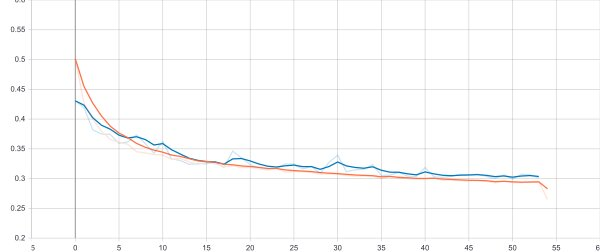
\includegraphics[height=3.4cm, keepaspectratio]{First_Model_CNN_Dec04_19-24-31_epoch_loss.jpg}
			\caption{CNN \texttt{loss} plot}
		\end{figure}
	
		\begin{figure}[H]
			\centering
			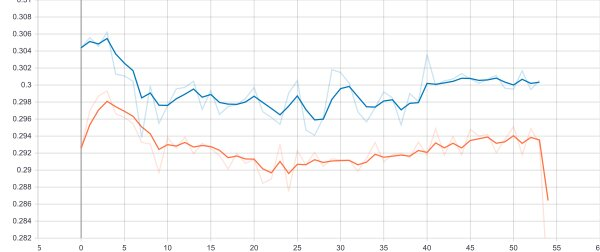
\includegraphics[height=3.4cm, keepaspectratio]{First_Model_CNN_Dec04_19-24-31_epoch_my_IoU.jpg}
			\caption{CNN \texttt{My\_IoU} plot}
		\end{figure}
			
		The graphs shows a sudden decrease because the training was interrupted before terminating.
		
		\subsection{First Model with concatenation}
			We tried to add concatenation to the model provided during the lab session. The setup did not change noticeably. This turned out in \texttt{train\_loss=0.250}, \texttt{valid\_loss=0.300} and \texttt{kaggle\_score=0.37682}.
			
			\begin{figure}[H]
				\centering
				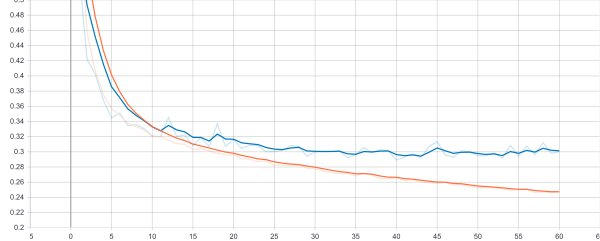
\includegraphics[height=3.4cm, keepaspectratio]{First_Model_conv_CNN_Dec06_20-49-34_epoch_loss.jpg}
				\caption{CNN with concatenation \texttt{loss} plot}
			\end{figure}
	
			\begin{figure}[H]
				\centering
				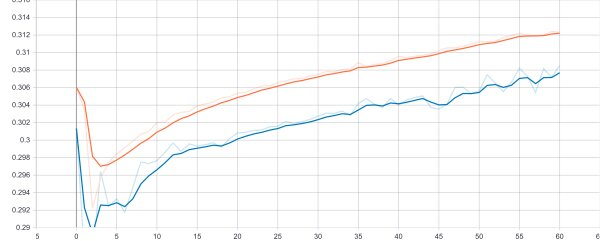
\includegraphics[height=3.4cm, keepaspectratio]{First_Model_conv_CNN_Dec06_20-49-34_epoch_my_IoU.jpg}
				\caption{CNN with concatenation\texttt{My\_IoU} plot}
			\end{figure}
			
	\section{UNet}
	
		We realized we were not applying concatenation correctly so we reimplemented a UNet style model using Keras Functional  API, explicitly declaring each layer. We used the same setup as before.  Here we realized the model was not performing as good as we expected, the graphs showed that the model was not learning.
		This started a series of attempts to change the model hyperparameters. 
		Our best attempt resulted in \texttt{train\_loss=0.21}, \texttt{val\_loss=0.31} and \texttt{kaggle\_score=0.39594} 
		
		\begin{figure}[H]
			\centering
			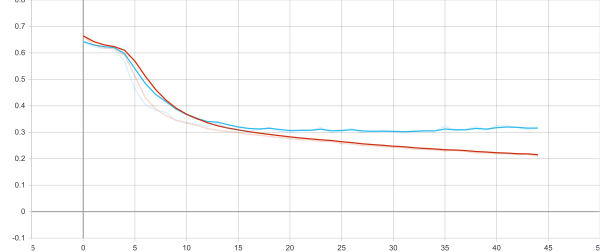
\includegraphics[height=3.4cm, keepaspectratio]{U-Net_conc_Dec07_14-23-41_epoch_loss.jpg}
			\caption{UNet \texttt{loss} plot}
		\end{figure}
	
		\begin{figure}[H]
			\centering
			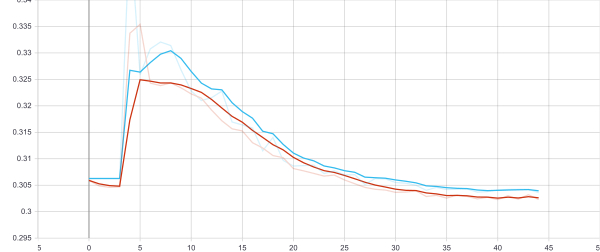
\includegraphics[height=3.4cm, keepaspectratio]{U-Net_conc_Dec07_14-23-41_epoch_my_IoU.jpg}
			\caption{UNet \texttt{My\_IoU} plot}
		\end{figure}
			
	\section{Failing attempts}
		
		The main issue with the model was that it went straight to a local optimum with \texttt{train\_loss=0} and \texttt{train\_my\_IoU=0}. \\
    	We noticed that the \texttt{num\_classes} parameter was used to define the number of filters in the last layer, since we needed just one image as prediction output we changed to \texttt{num\_classes=1}. \\
    	Adding Stochastic Gradient Descent to model optimizers slightly improved the model performances since it didn't immediately go down to \texttt{my\_IoU=0}.
	
		\subsection{Loss Functions}
			
			We thought the model was going into a local optimum due to the loss function we were using. To overcome this problem we tried different loss functions. 
			
			\subsubsection{Binary Cross Entropy}
				
				The Cross Entropy loss functions measures the accuracy of the network over each single pixel.
				
				\[\text{CE}\left(p, \hat{p}\right) = -\left(p \log\left(\hat{p}\right) + (1-p) \log\left(1 - \hat{p}\right)\right)\]		
			
			\subsubsection{Dice Loss}
				
				The Dice loss gives a feedback closely related to IoU. It measures the average prediction accuracy over the target instead of looking at the precision of single pixels.
			
				\[\text{DC} = \frac{2 TP}{2 TP + FP + FN} = \frac{2|X \cap Y|}{|X| + |Y|}\]
				
				\begin{itemize}
					\item TP = True Positives
					\item FP = False Positives
					\item FN = False Negatives
					\item X = Prediction
					\item Y = Target
				\end{itemize}
			
			\subsubsection{Combined Loss}
				We decided to use Binary Cross Entropy in combination with Dice Loss, giving the same weight to both, in order to find a model able to identify high-level features and achieve good accuracy at a local scale.
				
		\subsection{Dataset Split}
			Following the advise of tutor Lattari we changed our dataset split method and rolled back to the \texttt{ImageDataGenerator} built-in \texttt{validation\_split} feature. This showed immediate improvements meaning we had some errors in the code used to split the dataset. 
		
	\section{Transfer Learning}
		
		All the previous attempts we tried on the last model turned out in very low Kaggle scores. This meant we had a very low performing model so we tried to implement Transfer Learning.
		
		\subsection{VGG16}
			
			We used VGG16 as Encoder with fine-tuning of last six layers and the UNet Keras-Functional-API implementation Decoder mentioned before. We used Combined Loss as loss function. \\
			This model ended with \texttt{train\_loss=0.4653}, \texttt{valid\_loss=0.5639} and \texttt{kaggle\_score=0.47406}.
			
		\begin{figure}[H]
			\centering
			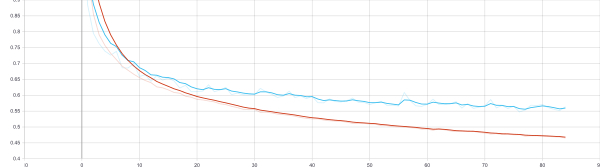
\includegraphics[height=3.4cm, keepaspectratio]{VGG16_Dec14_16-52-56_epoch_loss.jpg}
			\caption{VGG16 \texttt{loss} plot}
		\end{figure}
	
		\begin{figure}[H]
			\centering
			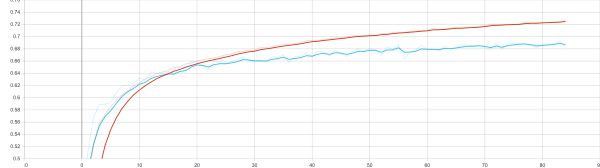
\includegraphics[height=3.4cm, keepaspectratio]{VGG16_Dec14_16-52-56_epoch_my_IoU}
			\caption{VGG16 \texttt{My\_IoU} plot}
		\end{figure}
			
		\subsection{VGG16 with concatenation}
					
			We implemented VGG16 using Keras Functional API and initiliazed the model with downloaded weights. 
		
		\subsection{VGG19 with concatenation}
		
			We repeated the attempt with a more recent architecture.
			
			
\end{document}
